\documentclass[a4paper,11.5pt,]{article}
\usepackage[utf8]{inputenc}
\usepackage[T1]{fontenc,url}
\usepackage[english,]{babel}
\usepackage{blindtext}
\usepackage{natbib}
\usepackage{gensymb}
\usepackage{amsmath}
\usepackage{changepage}
\usepackage{amssymb}
\usepackage{commath}
\usepackage{physics}
\usepackage{multicol}
\usepackage{float}
\usepackage{listings}
\usepackage{graphicx}
\usepackage{hyperref}
\usepackage{svg}
\usepackage{wrapfig}

\newenvironment{Figure}
  {\par\medskip\noindent\minipage{\linewidth}}
  {\endminipage\par\medskip}

\usepackage{multicol}
%\setlength{\columnsep}{1cm}

\usepackage{geometry}
 \geometry{
 a4paper,
 total={170mm,257mm},
 textheight =  592mm,
 left=20mm,
 right=20mm,
 tmargin=20mm,
 bmargin=20mm
 }
 \setlength{\columnsep}{20pt}
          

 \title{Stellar Spectra A. - Basic Line Formation\\
 AST4310}
 \date{\normalsize{14. September 2018} }
 \author{\textsc{\small{Metin San}}}
 
 
\begin{document}

\maketitle
\begin{center}
\textsc{Introduction}
\end{center}


\begin{adjustwidth}{1cm}{1cm}

Spectral lines in stellar spectra make out the foundation of astrophysics. They provide a wealth of knowledge about the studied object and are therefore one of the most valuable sources of information to an astrophysicist. In order to get an understanding of spectral lines we will follow the work of Cecilia Payne and Marcel Minnaert which are some of the early pioneers of spectral astronomy. The report is split into two parts. The first part considers Saha-Boltzmann modeling with Cecilia Payne, while the second part deals with Fraunhofer lines and their strenghts with Marcel Minnaert.
\end{adjustwidth}
\begin{multicols}{2}

\begin{center}
\textsc{1. The Boltzmann and Saha laws}
\end{center}
Cecilia Payne (1900 - 1979) was a British-American astronomer and astrophysicist famous for showing that most stars are made of mainly hydrogen and helium. She applied the Saha distribution which was newly derived to stellar spectra. With this she was able to show that the empirical Harvard classification primarily represented a temperature scale.

In thermodynamical equilibrium, the equipartition laws Saha and Boltzmann describe the division of particles of a specific element. With the temperature as the only major parameter these laws show us how the different ionization stages and discrete energy levels of a specific element are distributed.

\begin{center}
1.1 \textit{Boltzmann distribution}
\end{center}
The Boltzmann distribution deals with the energy levels and is given by
\begin{equation}\label{eq:1}
    \frac{n_{r,s}}{N_r} = \frac{g_{r,s}}{U_r} e^{-\chi_{r,s}/kT},
\end{equation}
where $n_{r,s}$ is the number density (also called level population) and $g_{r,s}$ the statistical weight of the level $(r,s)$ where $r$ is the ionization stage, and $s$ is the state or level. $N_r = \sum_3 n_{r,s}$ is the total particle density over all levels of ionization. $\chi_{r,t}$ is the excitation energy measured from the ground state ($r,s=1$). The partition function $U_r$ is defined by

\begin{equation}\label{eq:2}
    U_r = \sum_s g_{r,s} e^{-\chi_{r,s}/kT}.
\end{equation}

\begin{center}
1.2 \textit{Strength ratio of $\alpha$ lines in hydrogen}
\end{center}
Payne was studying the absorption lines in stellar spectra when she made the assumption that the strength of the absorption lines scaled with the population density of the lower level of the corresponding transition. If one assumes that most of the hydrogen resides in the lower energy levels, it follows that most transitions would result in higher energy levels. The strength of the lines should therefore scale with the population density of these lower levels. We know today that this is assumption is completely correct, but stellar absorption lines do generally scale with larger lower-level populations. We will therefore proceed by assuming that Payne's assumption holds and that the scaling is linear.

This assumption allows us to estimate the strength ratios of the $\alpha$ lines of hydrogen, where $\alpha$ denotes that the excitation is from $s$ to $s+1$.  For a neutral hydrogen atom ($r = 1$), the statistical weight goes as $g_{1,s} = 2s^2$, and the excitation energy goes as $\chi_{1,s} = 13.6 (1- 1/s^2)$. The ratio between Lyman $\alpha$ ($s=1$) and Balmer $\alpha$ ($s=2$) is then given from the Boltzmann equation \eqref{eq:1} as

\begin{equation}\label{eq:3}
    \frac{n_{1,1}}{n_{1,2}} = \frac{g_{1,1}e^{-\chi_{1,1}/kT}}{g_{1,2} e^{-\chi_{1,2}/kT}},
\end{equation}
where $U_r$ and $N_r$ have canceled out. We only need to insert for $s$ and $g$ in order to compare. By using the formula in equation \eqref{eq:3} we can compute the strength ratio of the $\alpha$ lines in H I Lyman, Balmer, Paschen and Brackett series. For neutral hydrogen, the information need is tabulated in table \ref{tab:1}. Using the information in this table we find that the following strength ratios for the solar temperature of 5770 K: (Lyman $\alpha$ / Balmer $\alpha$) $\approx 2 \cdot 10^8$, (Balmer $\alpha$ / Paschen $\alpha$) $\approx $ 20, and (Balmer $\alpha$ / Brackett $\alpha$) $\approx 42$. We see that Lyman $\alpha$ line strength is enormous compared to the other lines. This is a result of the excitation energy $chi_{1,1} = 0$, making it temperature independent when computing ratios.

\begin{table}[H]
\begin{center}
\begin{tabular}{llll}
\hline
Line $\alpha$ & $s$ & $\chi_{1,s} $ {[}eV{]} & $g_{1,s}$ \\ \hline
Lyman         & 1   & 0                      & 2          \\
Balmer        & 2   & 10.20                  & 8          \\
Paschen       & 3   & 12.09                  & 18         \\
Brackett      & 4   & 12.75                  & 32         \\ \hline

\end{tabular}
\caption{Neutral hydrogen information}
\label{tab:1}
\end{center}
\end{table}





\begin{center}
1.3\textit{ Saha distribution}
\end{center}
The Saha distribution relates the ionization levels of an element in ionization equilibrium and is given by

\begin{equation}\label{eq:4}
    \frac{N_{r+1}}{N_r} = \frac{1}{N_e} \frac{2U_{r+1}}{U_r} \left( \frac{2\pi m_e k T}{h^2} \right)^{3/2} e^{-\chi_r /kT},
\end{equation}
where $m_e$ is the electron mass, $h$ is Planck's constant $N_e$ is the electron density, and $\chi_r$ is the threshold ionization energy required to ionize from stage $r$ to $r+1$.

\begin{center}
1.4\textit{ Element E (Schadeenium)}
\end{center}
We will now consider the imaginary element E, or "Schadeenium". E is a simple atom which lets us evaluate Saha-Boltzmann statistics without having to bother about complex atomic data. It has the following properties:
\begin{itemize}
    \item The statistical weight is $g_{r,s} = 1$ for all levels.
    \item For neutral E, the ionization energy is $\chi_1 = 7$ eV. For $E^+$ (ionized once) the energy is $\chi_2 = 16$ eV, and similarly $\chi_3 = 31$ eV and $\chi_4 = 51$ eV.
    \item The excitation energies increase incrementally by 1 eV: $\chi_{r,s} = s-1$ eV.
\end{itemize}

\noindent We begin by computing the partition function $U_r$ of E found in equation \eqref{eq:2}. The results is seen in figure \ref{fig:1}.

\begin{figure}[H]
	\centering
	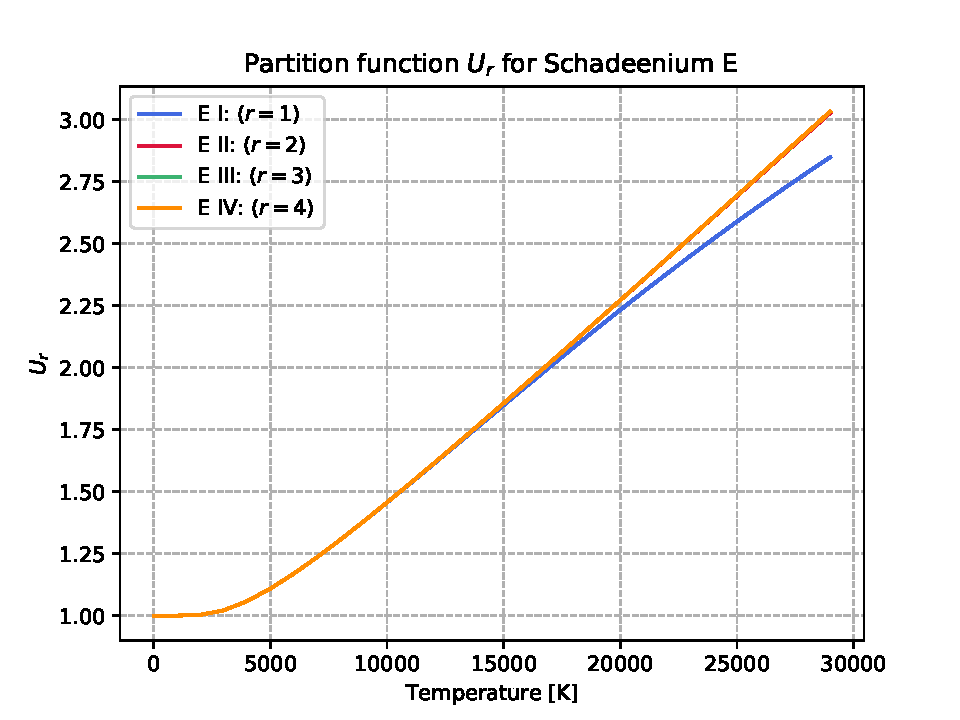
\includegraphics[width=0.5\textwidth]{figures/part_E.pdf}
	\caption{Partition function $U_r$ for the imaginary element E.}
	\label{fig:1}
\end{figure}

\noindent We find that all ionizations mostly behave the same way for temperatures below 15000 K. For higher temperatures, $U_1$ splits from the other ionizations and keeps a lower value. Generally we note that the partition function of element E is of order unity and appears to be weakly sensitive to temperature. 

Further we can compare our calculation with Schadee's first table. We find that for $T=5000$ K all ionizations have the value $U_r = 1.109$, which corresponds well to Schadee's $U_r = 1.11$. For $T = 10000$ K we find that again all ionizations have more or less the same value of $U_r = 1.456$, which can be rounded up to Schadee's $U_r = 1.46$. Finally for $T = 20000$ K we find that $U_1 = 2.232$ and $U_2 = U_3 = U_4 = 2.271$, where as Schadee tabulated $U_1 = 2.27$, and $U_2 = U_3 = U_4 = 2.27$. We see that these values correspond nearly perfectly to those tabulated by Schadee.

\begin{center}
1.4.1 \textit{ Boltzmann distribution for E}
\end{center}
With the partition function calculated, we can study the Boltzmann distribution for E. This is done by computing the boltzmann equation \eqref{eq:1} for varies levels $s$. The result can be seen in figure \ref{fig:2}.

\begin{figure}[H]
	\centering
	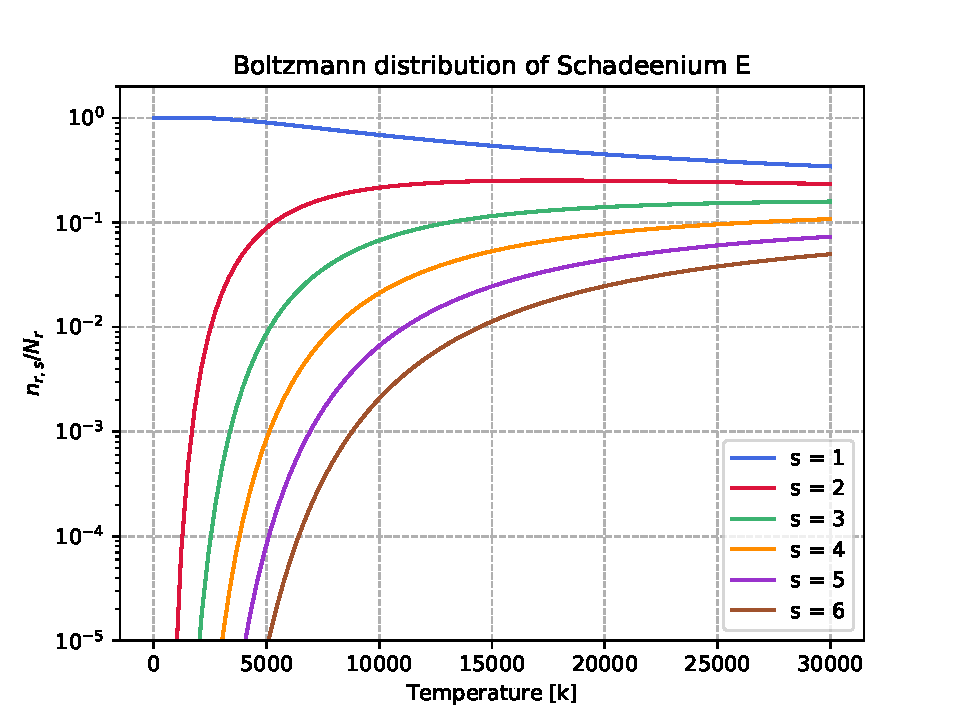
\includegraphics[width=0.5\textwidth]{figures/boltz_E.pdf}
	\caption{Boltzmann distribution of the imaginary element E.}
	\label{fig:2}
\end{figure}

\noindent By studying figure \ref{fig:2} we notice that in thermal equilibrium, for all temperatures, the ground state always has the largest population. At $T = 5000$ K we have $n_{r,s}/N_r = 0.9$ for $s = 1$ and $n_{r,s}/N_r \approx 0.009$ for $s=2$ and so on for the lower levels which perfectly corresponds to those tabulated by Schadee. We see that all these add up to unity for all temperatures, which is a results off the scaling by $N_r$. We can conclude that the lowest levels are the most important ones which is a result of the rapid decay of the Boltzmann factor $e^{-\chi_{r,s}/kT}$. This can also explain the insensitivity of $U_r$ to temperature. 

\begin{center}
1.4.2\textit{ Saha distribution for E}
\end{center}
We will now study the Saha distribution of the element E. By computing the saha equation \eqref{eq:4} for varying ionizations we obtain the results seen in figure \ref{fig:3}. Since this is a normalized distribution in the same way as the Boltzmann distribution, the ionizations always add up to one. We also notice that for solar temperatures, only 2 ionizations are significantly present. At $T = 5000$ we see that $N_{r+1}/N_r \approx 0.91$ for $r = 1$, while  $N_{r+1}/N_r \approx 0.089$ for $r = 2$, while the higher ionization stages are negligible. This means that for solar temperatures, E is mostly neutral. For higher temperatures around $T = 10000$ K, we find that $N_{r+1}/N_r \approx 0.95$ for $r = 2$ and $N_{r+1}/N_r \approx 0.05$ for $r = 3$, while the other ionizations are again negligible. These values correspond nicely to those found by in Schadee's table. This suggests that there are at all times mainly 2 ionizations stages present in a gas at a given temperature.


\begin{figure}[H]
	\centering
	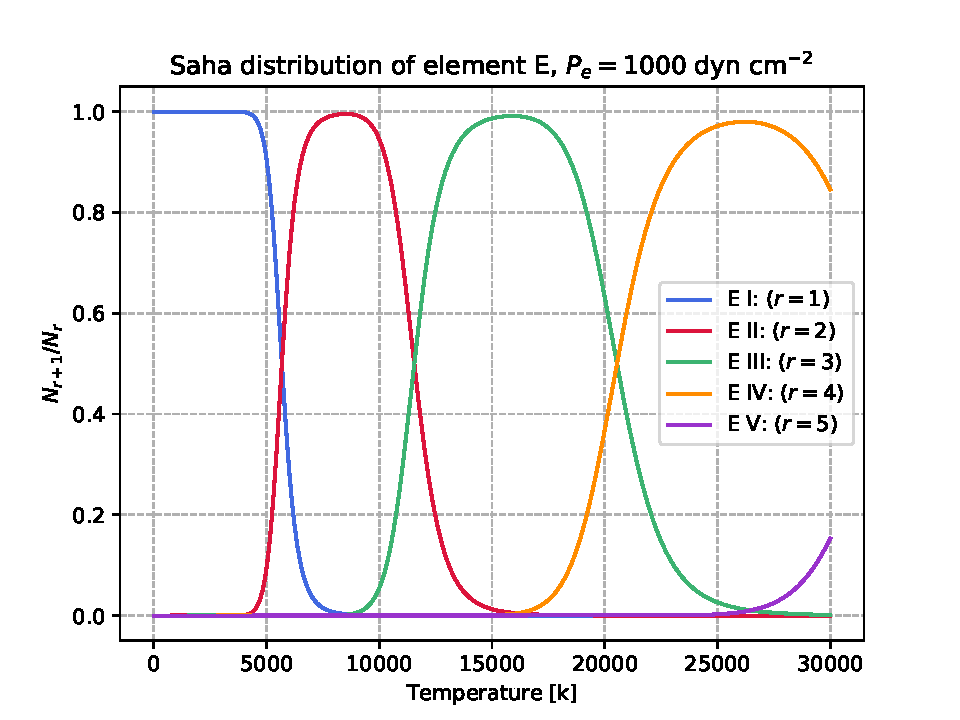
\includegraphics[width=0.5\textwidth]{figures/saha_E.pdf}
	\caption{Saha distribution of the imaginary element E with an electron pressure of $P = 1000$ dyn cm$^{-2}$ .}
	\label{fig:3}
\end{figure}

We can also study what effects the electron pressure has on the saha distribution. We do so by computing the saha equation \eqref{eq:4} for two values of $P_e$. The results of this can be seen in figure figure \ref{fig:4}.


\begin{figure}[H]
	\centering
	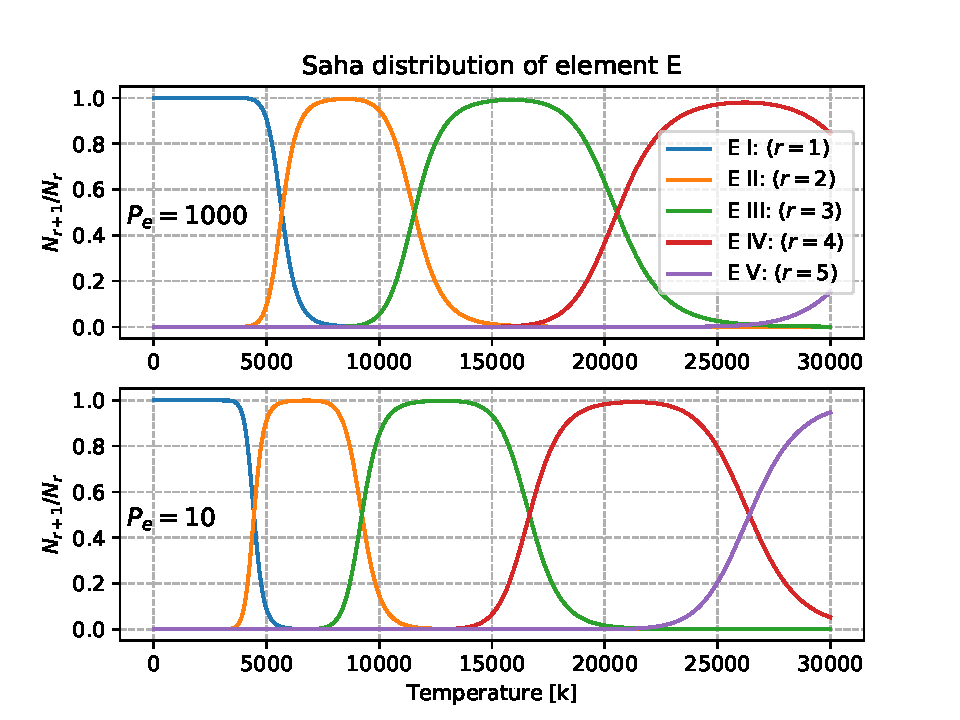
\includegraphics[width=0.5\textwidth]{figures/saha_sub.pdf}
	\caption{Saha distribution of the imaginary element E for two different electron pressures. Upper plot: $P_e = 1000$. Lower plot: $P_e = 10$, where $P_e$ has units [dyn cm$^{-2}$].}
	\label{fig:4}
\end{figure}

Figure \ref{fig:4} shows the difference $P_e$ makes when computing the Saha distribution. We note that in the lower subplot with $P_e = 10$ the distribution seems to have been squished towards the left. This means that ionization occurs at earlier temperatures for low values of electron pressure.

We note that the Boltzmann and Saha distributions behave differently for increasing temperatures. The Boltzmann equation converges to to $g_{r,s}/U_r$ as $T \rightarrow \infty$. The same is not true for the Saha distribution. The two distributions share the term $e^{-\chi /kT}$ term which converges to 1 as $T \rightarrow $. However, the Saha distribution has a factor $T^{3/2}$ which grows exponentially as $T$ increases. This is the factor that separates the two distributions.

\begin{center}
1.4.3\textit{ Payne curves for E}
\end{center}
The underlying premise in Payne's analysis was that one might expect that the observed strength of a spectral line involving level ($r,s$) scales with the Saha-Boltzmann prediction for the lower level population $n_{r,s}$ (if Thermodynamical equilibrium holds in a stellar atmosphere). We will study this as Payne did by computing the product of the two distributions in question and then plotting the results in a Payne-like graph. 

We start by computing and plotting the ground state populations ($s=1$) for E with an electron pressure of $P_e = 131$ dyn cm$^2$. The result is seen in figure \ref{fig:5}

\begin{figure}[H]
	\centering
	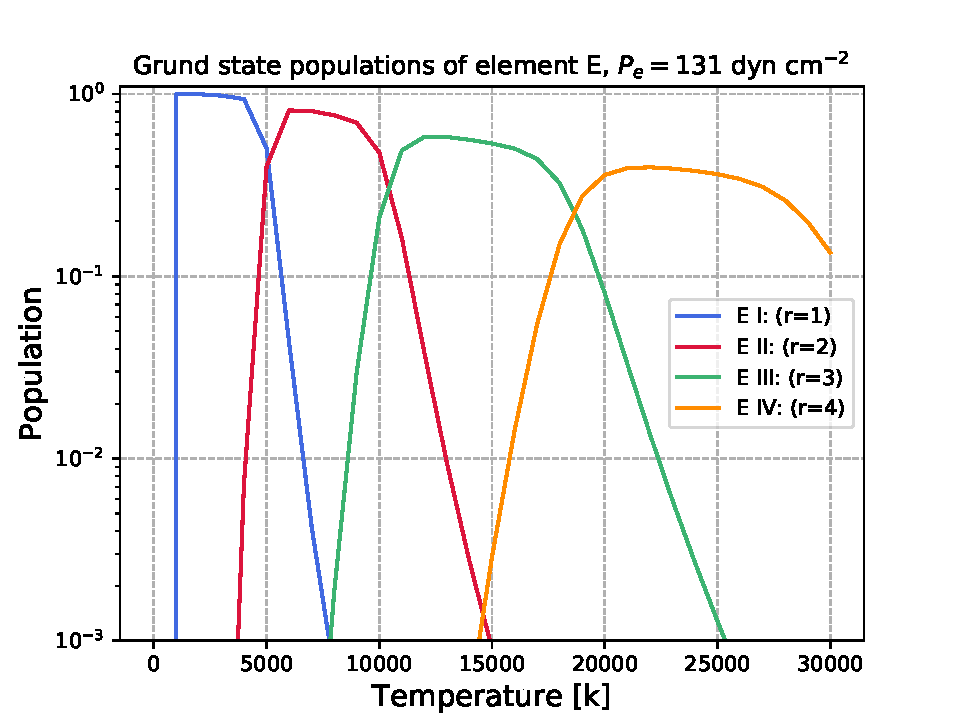
\includegraphics[width=0.5\textwidth]{figures/payne_E.pdf}
	\caption{Saha-Boltzmann distribution ground state populations for E.}
	\label{fig:5}
\end{figure}
\noindent Figure \ref{fig:5} shows the so called Payne curves of the ground state population of E. Its easy to recognize that this plot as a product of the Saha and Boltzmann distributions. We note that the maximum amplitude decreases with increasing ionization which is a result of the Boltzmann distribution. The steep flanks on the left and right side are a result of the Saha distribution behaviour. We also see that the flanks get less steep as $T \rightarrow \infty$ which is also the case in the Saha distribution seen in \ref{fig:4}. The consequence of these steep flanks are that the probability of finding an unionized E I atom at temperatures above 10000 K is approximately 0. Similarely, for temperatures greater than 15000 K, most if not all atoms will be E II.
\begin{figure}[H]
	\centering
	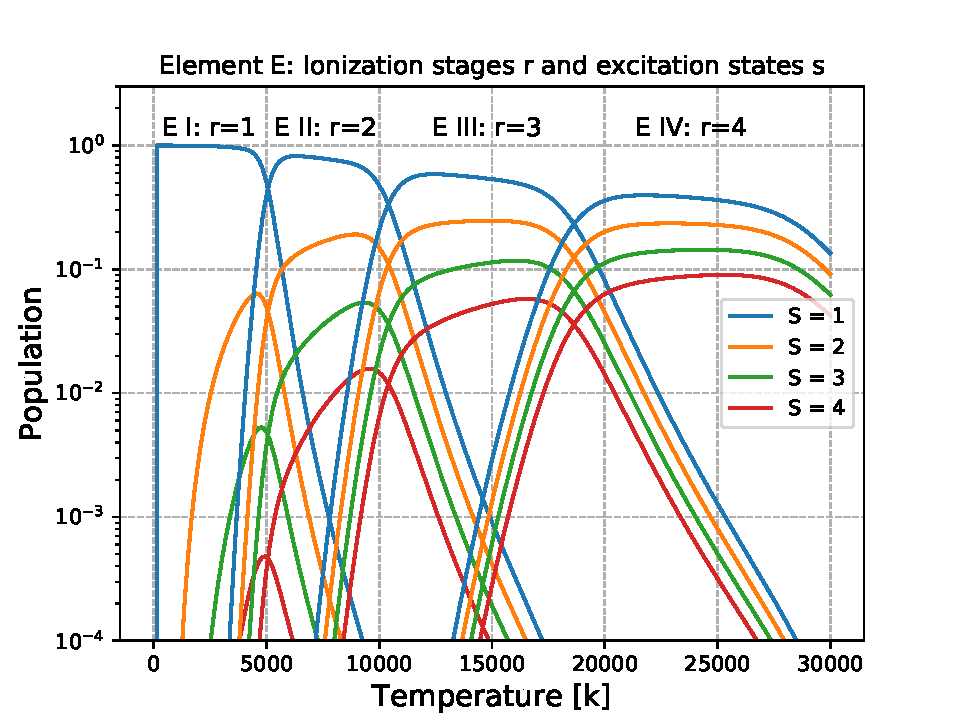
\includegraphics[width=0.5\textwidth]{figures/payne_E_multi.pdf}
	\caption{Payne curves for element E for various energy levels $s$. }
	\label{fig:6}
\end{figure}

\noindent We will now further study the influence of the Boltzmann factor by adding curves of higher values of excitation states $s$. By including excitation levels up to $s=4$, we find the following result seen in figure \ref{fig:6}. First of all we notice that the ground state ($s=1$) dominate the population for all ionizations and across all temperatures. However, as $T \rightarrow \infty$ the ground state population of the different ionizations gets smaller, meaning that the population is distributed more evenly over the different states.

These results resemble Payne's curves closely, which can be seen in figure 

\begin{figure}[H]
	\centering
	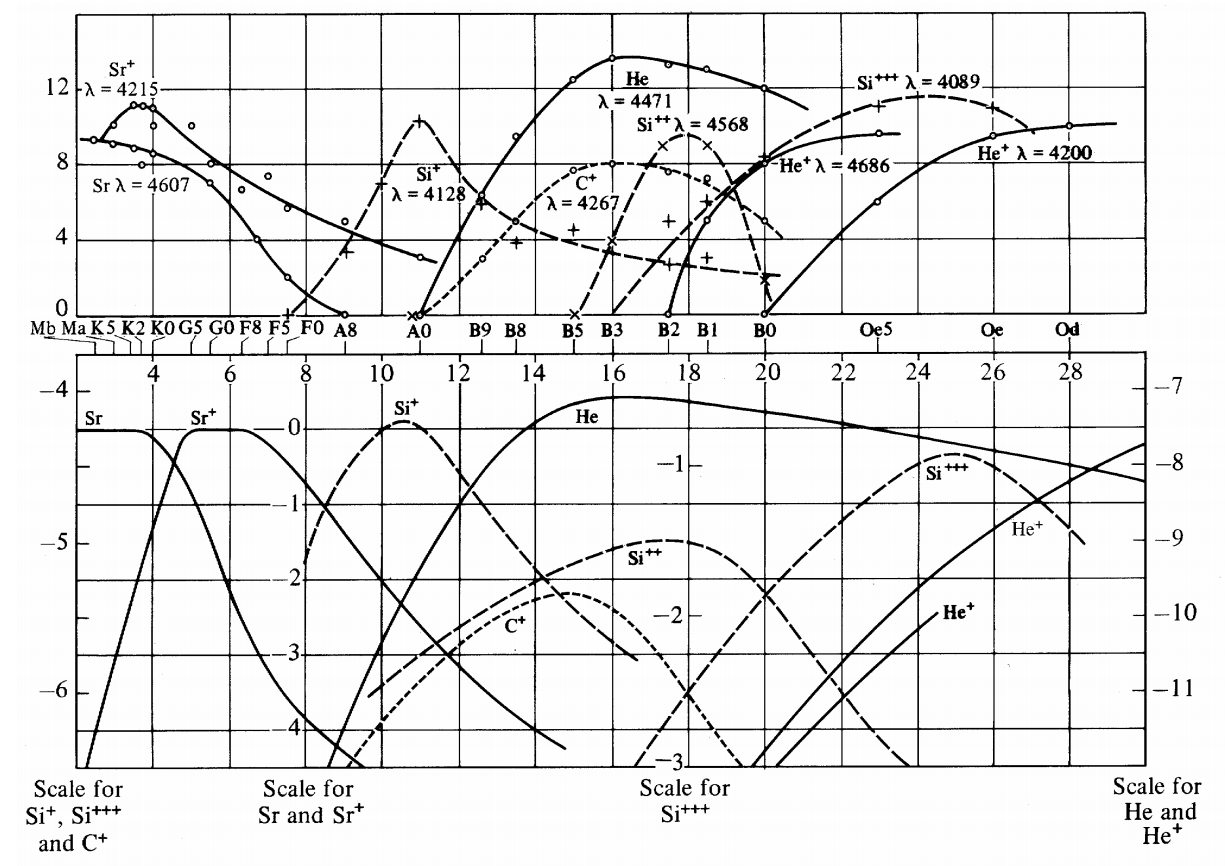
\includegraphics[width=0.5\textwidth]{SSA/figures/Payne.png}
	\caption{The original Payne curves (\textit{1924}). Upper panel displays the variations of observed line strengths. Lower panel displays the Saha-Boltzmann distribution.}
	\label{fig:7}
\end{figure}

Our produced results in figure \ref{fig:6} are comparable to those of Payne seen in the lower panel of \ref{fig:7}. In order to reproduce her results more closely we would need to evaluatute the equations for the actual elements she used instead of E. Her results are plotted as a function of the Harvard classification of stellar spectra, while our is a function of temperature. Payne's conclusion was therefore that the Harvard classification is primarily an ordering of temperature based on the Saha-Boltzmann population statistics.

\begin{center}
1.5\textit{ Hydrogen H I}
\end{center}
We will now extend our Saha-Boltzmann analysis to neutral hydrogen H I. Hydrogen is a bit more complex than the imaginary element E, but still fairly simple. It has the following properties

\begin{itemize}
    \item Ionization energy $ \chi_1 = 13.598$ eV
    \item Statistical weight $g_{1,s} = 2 s^2$
    \item Level energy $\chi_{1,s} = 13.598(1 - 1/s^2)$ eV
    \item Single ion stage $U_2 = g_{2,1} = 1$
\end{itemize}

\noindent In addition to hydrogen, we will also study the calcium line Ca$^+$ K. The Ca$^+$ K line behaves in the same way as element E for $r=2$ and $s=1$ with an exception of a factor 2 which makes for an easy calculation as we already have the Saha-Boltzmann routine for E.

\begin{center}
1.5.1\textit{ Saha-Boltzmann population of H I and Ca$^+$ K}
\end{center}

\noindent By using the new information for Hydrogen and Ca$^+$, we have computed the Saha-Boltzmann distribution which can be seen in figure \ref{fig:8}

\begin{figure}[H]
	\centering
	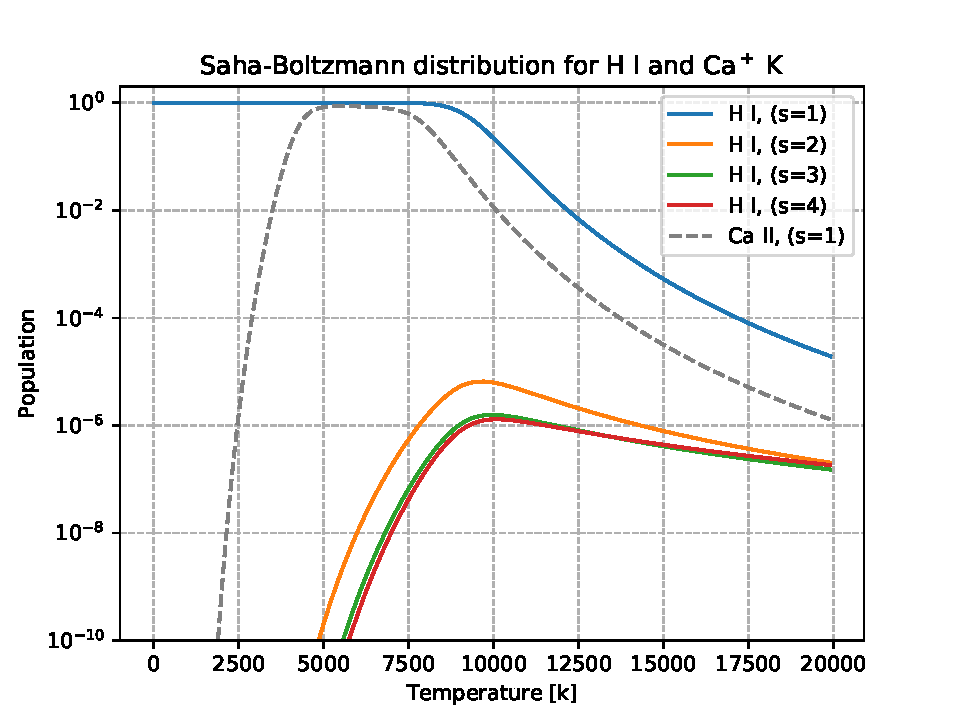
\includegraphics[width=0.5\textwidth]{SSA/figures/sahabolt_HCA.pdf}
	\caption{Saha-Boltzmann distribution of H I and Ca$^+$ K.}
	\label{fig:8}
\end{figure}

\noindent We will ignore the Ca$^+$ K population to begin with. By comparing the Saha-Boltzmann distribution for H I and E I, seen in figure \ref{fig:6}, we see that there are some some similarities. The main difference being that H I seems to fall off more slowly for higher temperatures.

\begin{center}
1.5.2\textit{ Solar H $\alpha$ versus Ca$^+$ K: Line strength}
\end{center}
If one studies the spectrum of the sun, as Payne did, one notices that the Ca$^+$ K spectral line is much stronger than the hydrogen $\alpha$ lines. This is strongly contradictory to the previous assumption made which says that the strength of the absorption lines scaled with the population density as one knows that hydrogen is massively more abundant than calcium ($N_\text{Ca}/N_\text{H} = 2 \cross 10^{-6}$). 

However, the H $\alpha$ line is a $s = 2 \rightarrow 3$ transition, and by studying the Saha-Boltzmann distribution in figure \ref{fig:8} we see that the the H I $(S=2)$ abundance at solar temperatures is of order $10^{-10}$. The Ca$^+$ K has the ground state as its lower transition, and has therefore the dominating population, which means that the assumption still holds.

We can prove this by computing the expected strength ratio of these two lines as a function of temperature. We find this ratio by multiplying the calcium abundance with the Saha-Boltzmann ratio of the two elements. The result is then plotted in figure \ref{fig:9}. 

\begin{figure}[H]
	\centering
	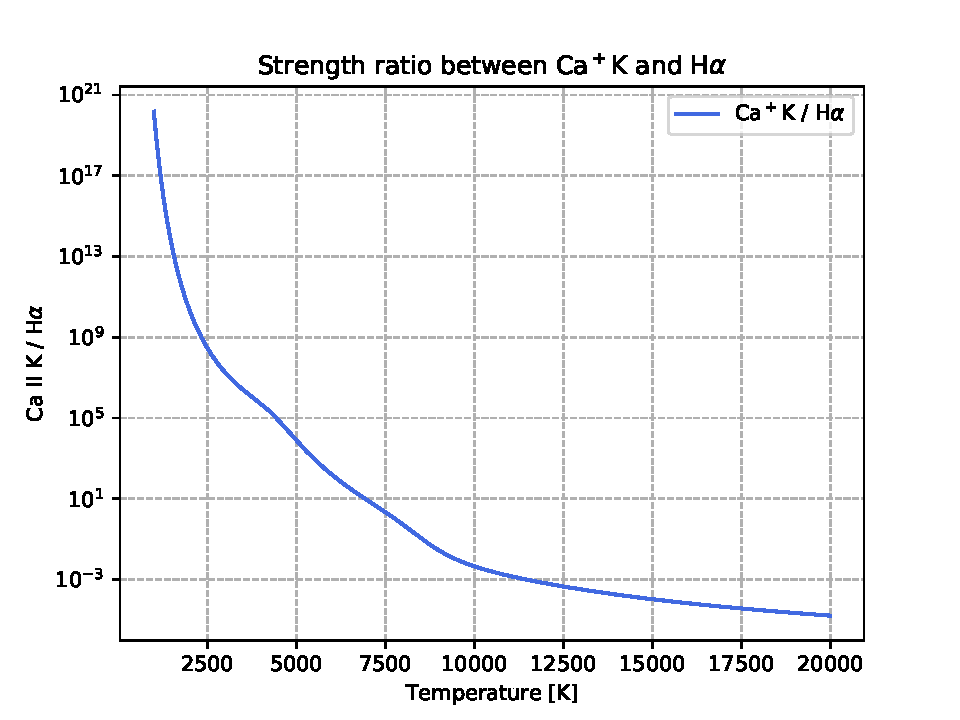
\includegraphics[width=0.5\textwidth]{SSA/figures/strengthratio.pdf}
	\caption{Solar line strength ratio Ca$^+$ K / H$\alpha$ with $P_e = 100$ dyn cm$^2$ }
	\label{fig:9}
\end{figure}

\noindent At low temperatures we observe a complete domination by the calcium line. However, we see that the ratio exponentially weakens as the temperature increases. This is expected as there are more and more hydrogen atoms that get ionized, which leads to a higher H II abundance. 

\begin{center}
1.5.3\textit{ H $\alpha$ vs Ca$^+$ K: Temperature sensitivity}
\end{center}
It is of interest to study how the two lines differ in their temperature sensitivity. We can do so by computing and plotting the relative population changes 
\[
\frac{(\Delta n_\text{Ca}/\Delta T)}{n_\text{Ca}} \quad \text{and} \quad \frac{(\Delta n_\text{H}/\Delta T)}{n_\text{H}},
\]
where $\Delta T$ is a small temperature change. The result can be seen in the upper panel in figure \ref{fig:10}, where we have also plotted each population in relative units in the lower panel.

\begin{figure}[H]
	\centering
	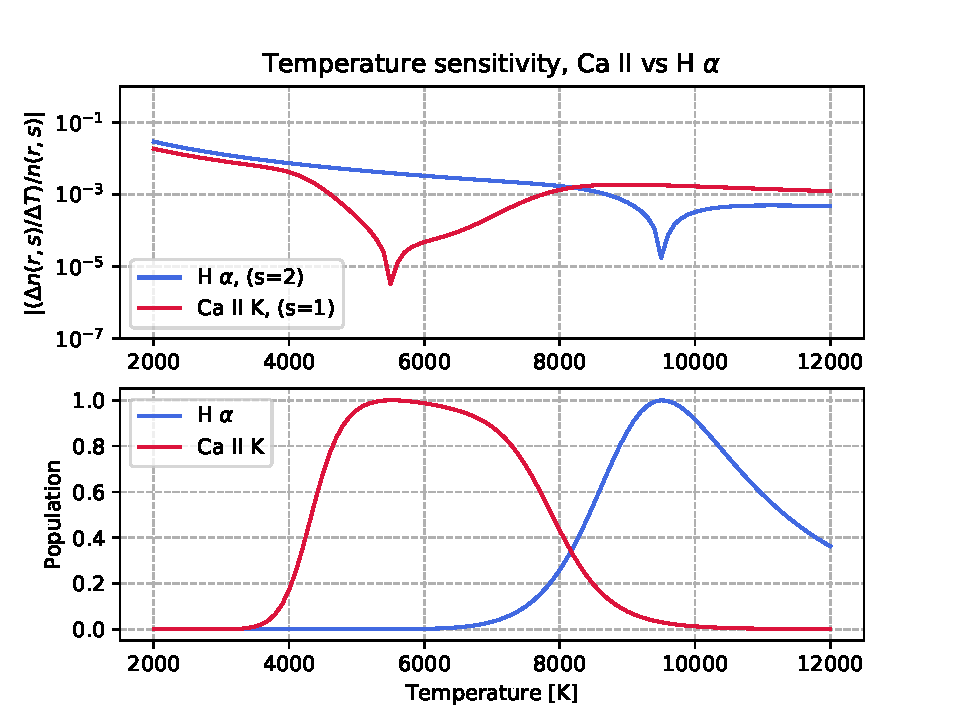
\includegraphics[width=0.5\textwidth]{SSA/figures/tempsens.pdf}
	\caption{Upper panel: Temperature sensitivity of Ca II and H $\alpha$. Lower panel: Relative population of the corresponding elements.}
	\label{fig:10}
\end{figure}
From figure \ref{fig:10} we notice that both lines start of with roughly the same sensitivity. We spot two dips in the temperature sensitivity. One for Ca II around 5 600 K, and one for H $\alpha$ around 9 500 K. The dips seem to occur once the population of each respective line reach their maxima. This can be interpreted as the sensitivity being at its highest when the population experience change. Similarly, the sensitivity experiences a rapid drop for the short temperature range where the population remains constant at the maxima.

The temperature sensitivity is essentially in some way the derivative of the population with respect to temperature. We see that the temperature sensitivity decreases at the left flank, so that $\Delta n < 0$, while the opposite is true at the right flank $\Delta n > 0$.

We also note that H $\alpha$ is the more temperature sensitive line for temperatures which corresponds to those of the solar photosphere.

\begin{center}
1.5.4\textit{ Hot stars versus cool stars}
\end{center}


\end{multicols}
\end{document}